{\color{gray}\hrule}
\begin{center}
\section{Experimental Evaluation}
\textbf{Analysis of YOLO's performance across biomedical and agricultural applications}
\bigskip
\end{center}
{\color{gray}\hrule}
\begin{multicols}{2}

\subsection{Experimental Setup}
In this section, we present a comprehensive evaluation of YOLO v11's performance in two distinct industries: biomedicine and agriculture. We examined three specific applications: COVID-19 detection using chest X-rays, blood cell detection and classification, and fruit ripeness determination. These applications were chosen to represent diverse real-world scenarios with varying levels of complexity, object characteristics, and practical significance.

\subsubsection{COVID-19 Chest X-ray Dataset}
For COVID-19 detection, we utilized the COVID-19 Image Dataset from Kaggle \citep{Raikokte2020}, which contains X-ray images categorized into three classes: COVID-19 positive cases, normal cases, and viral pneumonia cases. The dataset was prepared with particular attention to medical imaging requirements. Our dataset comprised 158 training images, 25 validation images, and 24 test images across three classes: Covid (0), Normal (1), and Viral Pneumonia (2). The images were grayscale chest X-rays with varying dimensions, and we converted annotations to YOLO format with central bounding boxes covering the regions of interest.

Given the specialized nature of medical imaging and the relatively small dataset size, we implemented careful training strategies to prevent overfitting while ensuring the model could detect subtle radiological patterns associated with COVID-19 infection.

\subsubsection{Blood Cell Detection Dataset}
For the blood cell detection task, we utilized the Blood Cell Detection dataset from Roboflow (version 3), containing microscopic images of blood samples with annotations for three types of blood cells. This comprehensive collection provided sufficient samples for robust training across three classes: Platelets, Red Blood Cells (RBC), and White Blood Cells (WBC). The dataset featured high-resolution microscopy images with clearly visible cellular structures and precise bounding box annotations around individual cells.

This dataset represents a challenging scenario for object detection due to the presence of numerous, often overlapping cells with varying sizes and the need for high precision in medical diagnostics.

\subsubsection{Fruit Ripeness Dataset}
For agricultural applications, we focused on fruit ripeness detection using the "Fruits Fresh and Rotten for Classification" dataset, containing images of fresh and rotten fruits of three different types. The dataset included six categories: Fresh Apple, Fresh Banana, Fresh Orange, Rotten Apple, Rotten Banana, and Rotten Orange. The RGB images captured individual fruits against various backgrounds with balanced representation across all six categories (approximately 1,500-2,200 instances per class).

To enhance the model's ability to detect ripeness-related features, we implemented a specialized Roughness-Local Binary Pattern (R-LBP) preprocessing technique that improved texture distinction between fresh and rotten fruits.

\subsubsection{Model Configurations}
We configured YOLO v11 differently for each application based on dataset characteristics and application requirements. For COVID-19 X-ray detection, we employed the YOLO v11m (medium) variant with 640×640 pixel input resolution, batch size of 16, and 20 training epochs. We used Adam optimizer with a learning rate of 1e-5 and implemented limited augmentation: rotation (0°), horizontal flip (0.5), translation (0.1), and scale (0.1). Notably, we disabled mosaic and mixup augmentations, which are typically unsuitable for medical images.

For blood cell detection, we utilized the larger YOLO v11l variant, maintaining the 640×640 pixel input resolution and batch size of 16, but extending training to 80 epochs with a learning rate of 0.01. We conducted training on a single NVIDIA A100 GPU and implemented standard augmentations including mosaic (1.0) and horizontal flip (0.5).

The fruit ripeness detection task employed the lightweight YOLO v11n (nano) variant with the same input resolution (640×640 pixels) and batch size (16), trained for 30 epochs. We applied our R-LBP technique for texture enhancement during preprocessing and utilized an optimizer auto-selected based on dataset characteristics.

Each configuration was chosen to optimize the model's performance for the specific task while considering computational efficiency and the unique characteristics of each dataset.

\subsection{Quantitative Results}
We evaluated each model's performance using standard object detection metrics: precision, recall, F1-score, mean Average Precision at 50\% IoU threshold (mAP@50), mean Average Precision across IoU thresholds from 50\% to 95\% (mAP@50-95), and inference speed in Frames Per Second (FPS).

To rigorously evaluate model performance across applications, we employed these metrics as defined mathematically:

\textbf{Precision}: $\text{Precision} = \frac{TP}{TP + FP}$

\textbf{Recall}: $\text{Recall} = \frac{TP}{TP + FN}$

\textbf{F1-Score}: $\text{F1-Score} = 2 \times \frac{\text{Precision} \times \text{Recall}}{\text{Precision} + \text{Recall}}$

\textbf{Mean Average Precision (mAP@IoU)}: The mean of the AP values across all classes at a specific IoU threshold.
\end{multicols}

\subsubsection{COVID-19 X-ray Detection Results}


\begin{table}[ht]
\centering
\begin{tabular}{|c|c|} \hline 

\textbf{Metric} & \textbf{Value} \\ \hline 

Precision & 0.7669 \\ \hline 
Recall & 0.3035 \\ \hline 
F1-Score & 0.4349 \\ \hline 
mAP@50 & 0.7263 \\ \hline 
mAP@50-95 & 0.6848 \\ \hline 
FPS & 33.76 \\ \hline

\end{tabular}
\caption{Overall Performance Metrics for COVID-19 X-ray Detection}
\label{tab:covid_results}
\end{table}


\begin{multicols}{2}
The YOLO v11m model showed promising performance on the COVID-19 X-ray dataset, as summarized in Table \ref{tab:covid_results}.

The class-wise performance analysis revealed significant variations across the three categories. The model performed best on the Normal class (class 1) with perfect precision (1.0) and a strong mAP@50 of 0.8278, while it struggled more with COVID-19 detection (class 0), achieving only 0.3035 recall despite a reasonable precision of 0.7669. Interestingly, the Viral Pneumonia class (class 2) showed a different pattern with high recall (0.8333) but lower precision (0.4713).
\end{multicols}

\begin{multicols}{2}
The confusion matrix analysis (Figure \ref{fig:covid_confusion}) indicated a tendency for the model to misclassify some COVID-19 cases as Viral Pneumonia, which is understandable given the radiological similarities between these conditions. This suggests that while the model has learned to distinguish normal X-rays effectively, it requires further refinement to reliably differentiate between pathological conditions with similar radiographic presentations.
\end{multicols}

\vspace{0.5in}

\begin{figure}[ht]
    \centering
    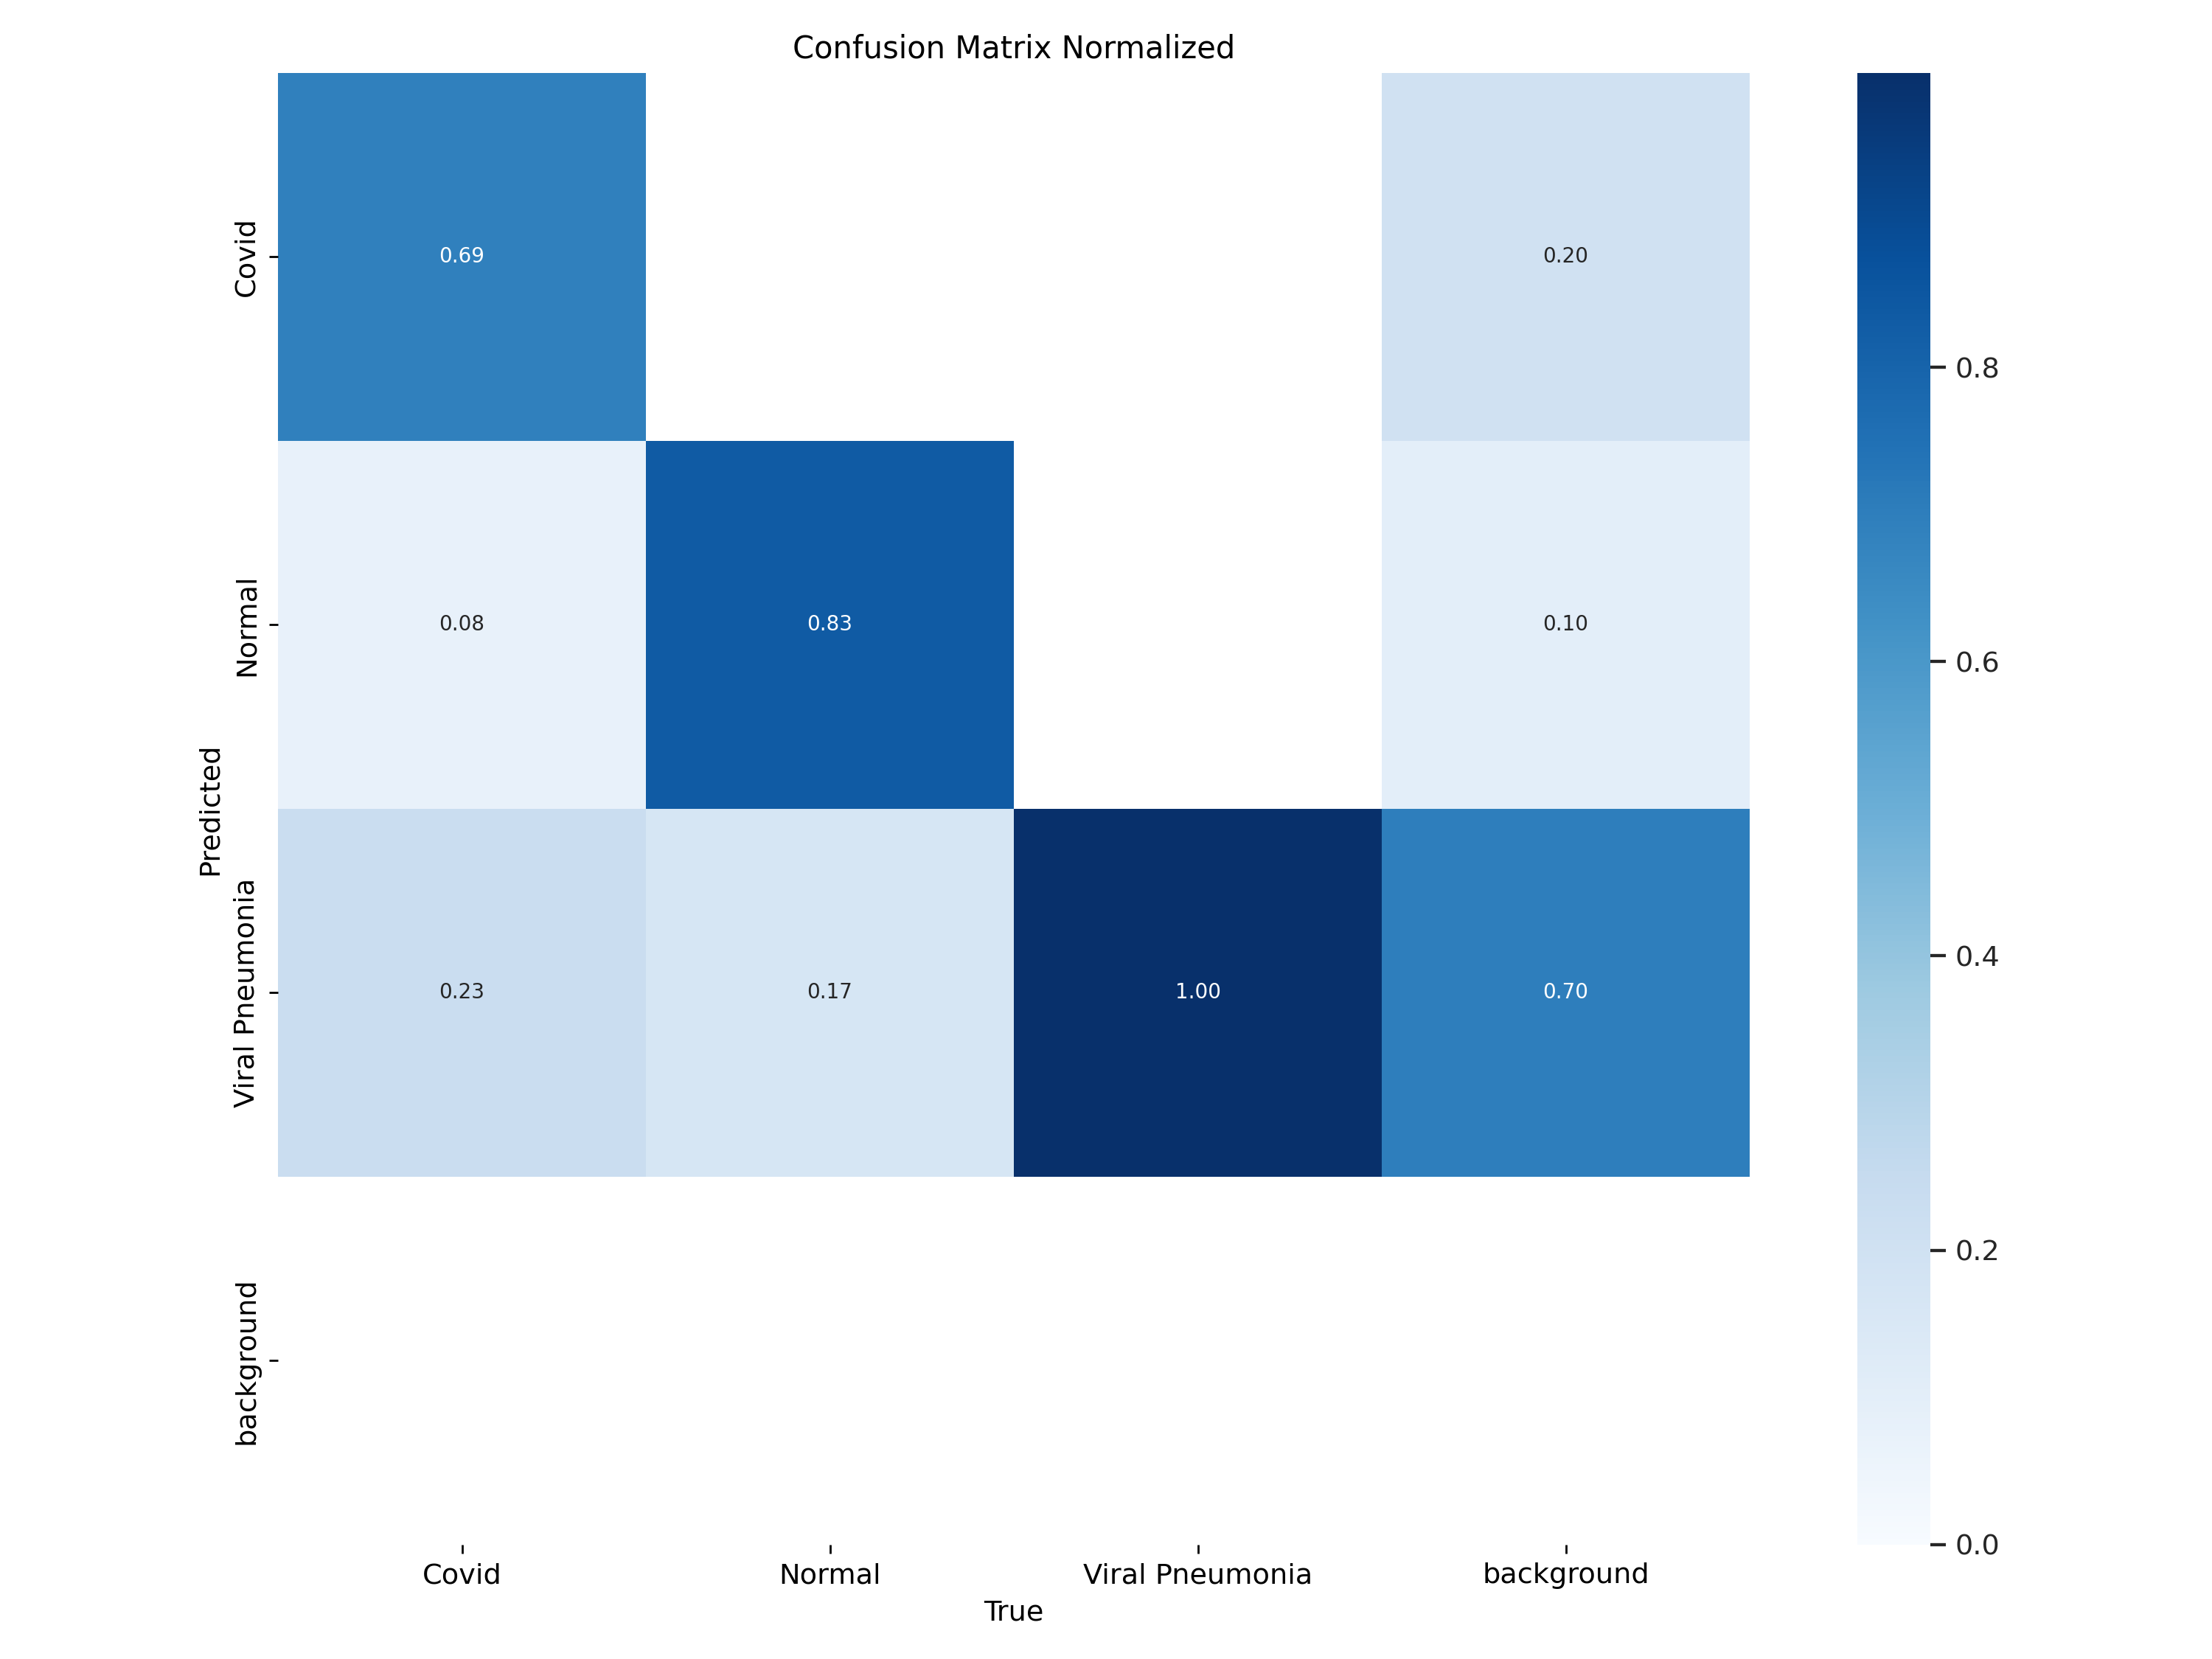
\includegraphics[width=1\textwidth]{datas/x_ray_summary_datas/x_ray_confusion_matrix_normalized.png}
    \caption{Result for Chest X-Ray Detection}
    \label{fig:covid_confusion}
\end{figure}

\vspace{0.5in}


\subsubsection{Blood Cell Detection Results}

\begin{table}[ht]
\centering
\begin{tabular}{|c|c|}
\hline
\textbf{Metric} & \textbf{Value} \\
\hline
Precision & 0.8560 \\
Recall & 0.9240 \\
F1-Score & 0.8887 \\
mAP@50 & 0.9340 \\
mAP@50-95 & 0.6770 \\
FPS & 38.45 \\
\hline
\end{tabular}
\caption{Overall Performance Metrics for Blood Cell Detection}
\label{tab:blood_cell_results}
\end{table}

\begin{multicols}{2}
The blood cell detection task yielded significantly better results, as detailed in Table \ref{tab:blood_cell_results}.

Class-wise analysis revealed that White Blood Cells (WBC) were detected with exceptional accuracy (precision: 0.952, recall: 1.000, F1-score: 0.975), likely due to their distinctive size and morphology. Red Blood Cells (RBC) proved more challenging with lower precision (0.736) but good recall (0.901), reflecting the difficulty in distinguishing individual RBCs in densely packed microscopy images. Platelets achieved balanced performance with precision and recall both around 0.87-0.88.
\end{multicols}

\begin{multicols}{2}
The superior performance on this dataset compared to the X-ray dataset can be attributed to several factors: (1) the larger dataset size providing more training examples, (2) the more distinctive visual characteristics of different blood cell types, and (3) the use of the larger YOLO v11l model variant with greater representational capacity.
\end{multicols}

\begin{figure}[ht]
\centering
\includegraphics[width=1\linewidth]{datas/blood_cell_summary_datas/blood_cells_detect.png}
\caption{Result for Blood Cell Detection}
\label{fig:blood_cell_class_metrics}
\end{figure}

\subsubsection{Fruit Ripeness Detection Results}

\begin{table}[ht]
\centering
\begin{tabular}{|c|c|}
\hline
\textbf{Metric} & \textbf{Value} \\
\hline
Precision & 0.9990 \\
Recall & 0.9997 \\
F1-Score & 0.9993 \\
mAP@50 & 0.9950 \\
Processing Time & ~5-7 ms/image (with GPU) \\
\hline
\end{tabular}
\caption{Overall Performance Metrics for Fruit Ripeness Detection}
\label{tab:fruit_results}
\end{table}

\begin{multicols}{2}
The fruit ripeness detection model achieved the most impressive results of all three applications, with near-perfect performance across all metrics, as shown in Table \ref{tab:fruit_results}.

The confusion matrix (Figure \ref{fig:fruit_confusion}) showed perfect classification accuracy for all six categories (Fresh Apple, Fresh Banana, Fresh Orange, Rotten Apple, Rotten Banana, and Rotten Orange), with no misclassifications observed. This exceptional performance can be attributed to:
\begin{enumerate}
    \item The highly distinctive visual differences between fresh and rotten fruits
    \item The effectiveness of the R-LBP preprocessing technique in enhancing texture features
    \item The well-balanced dataset with clear examples of each class
    \item The absence of overlapping objects or ambiguous cases
\end{enumerate}
\end{multicols}

\begin{figure}[ht]
\centering
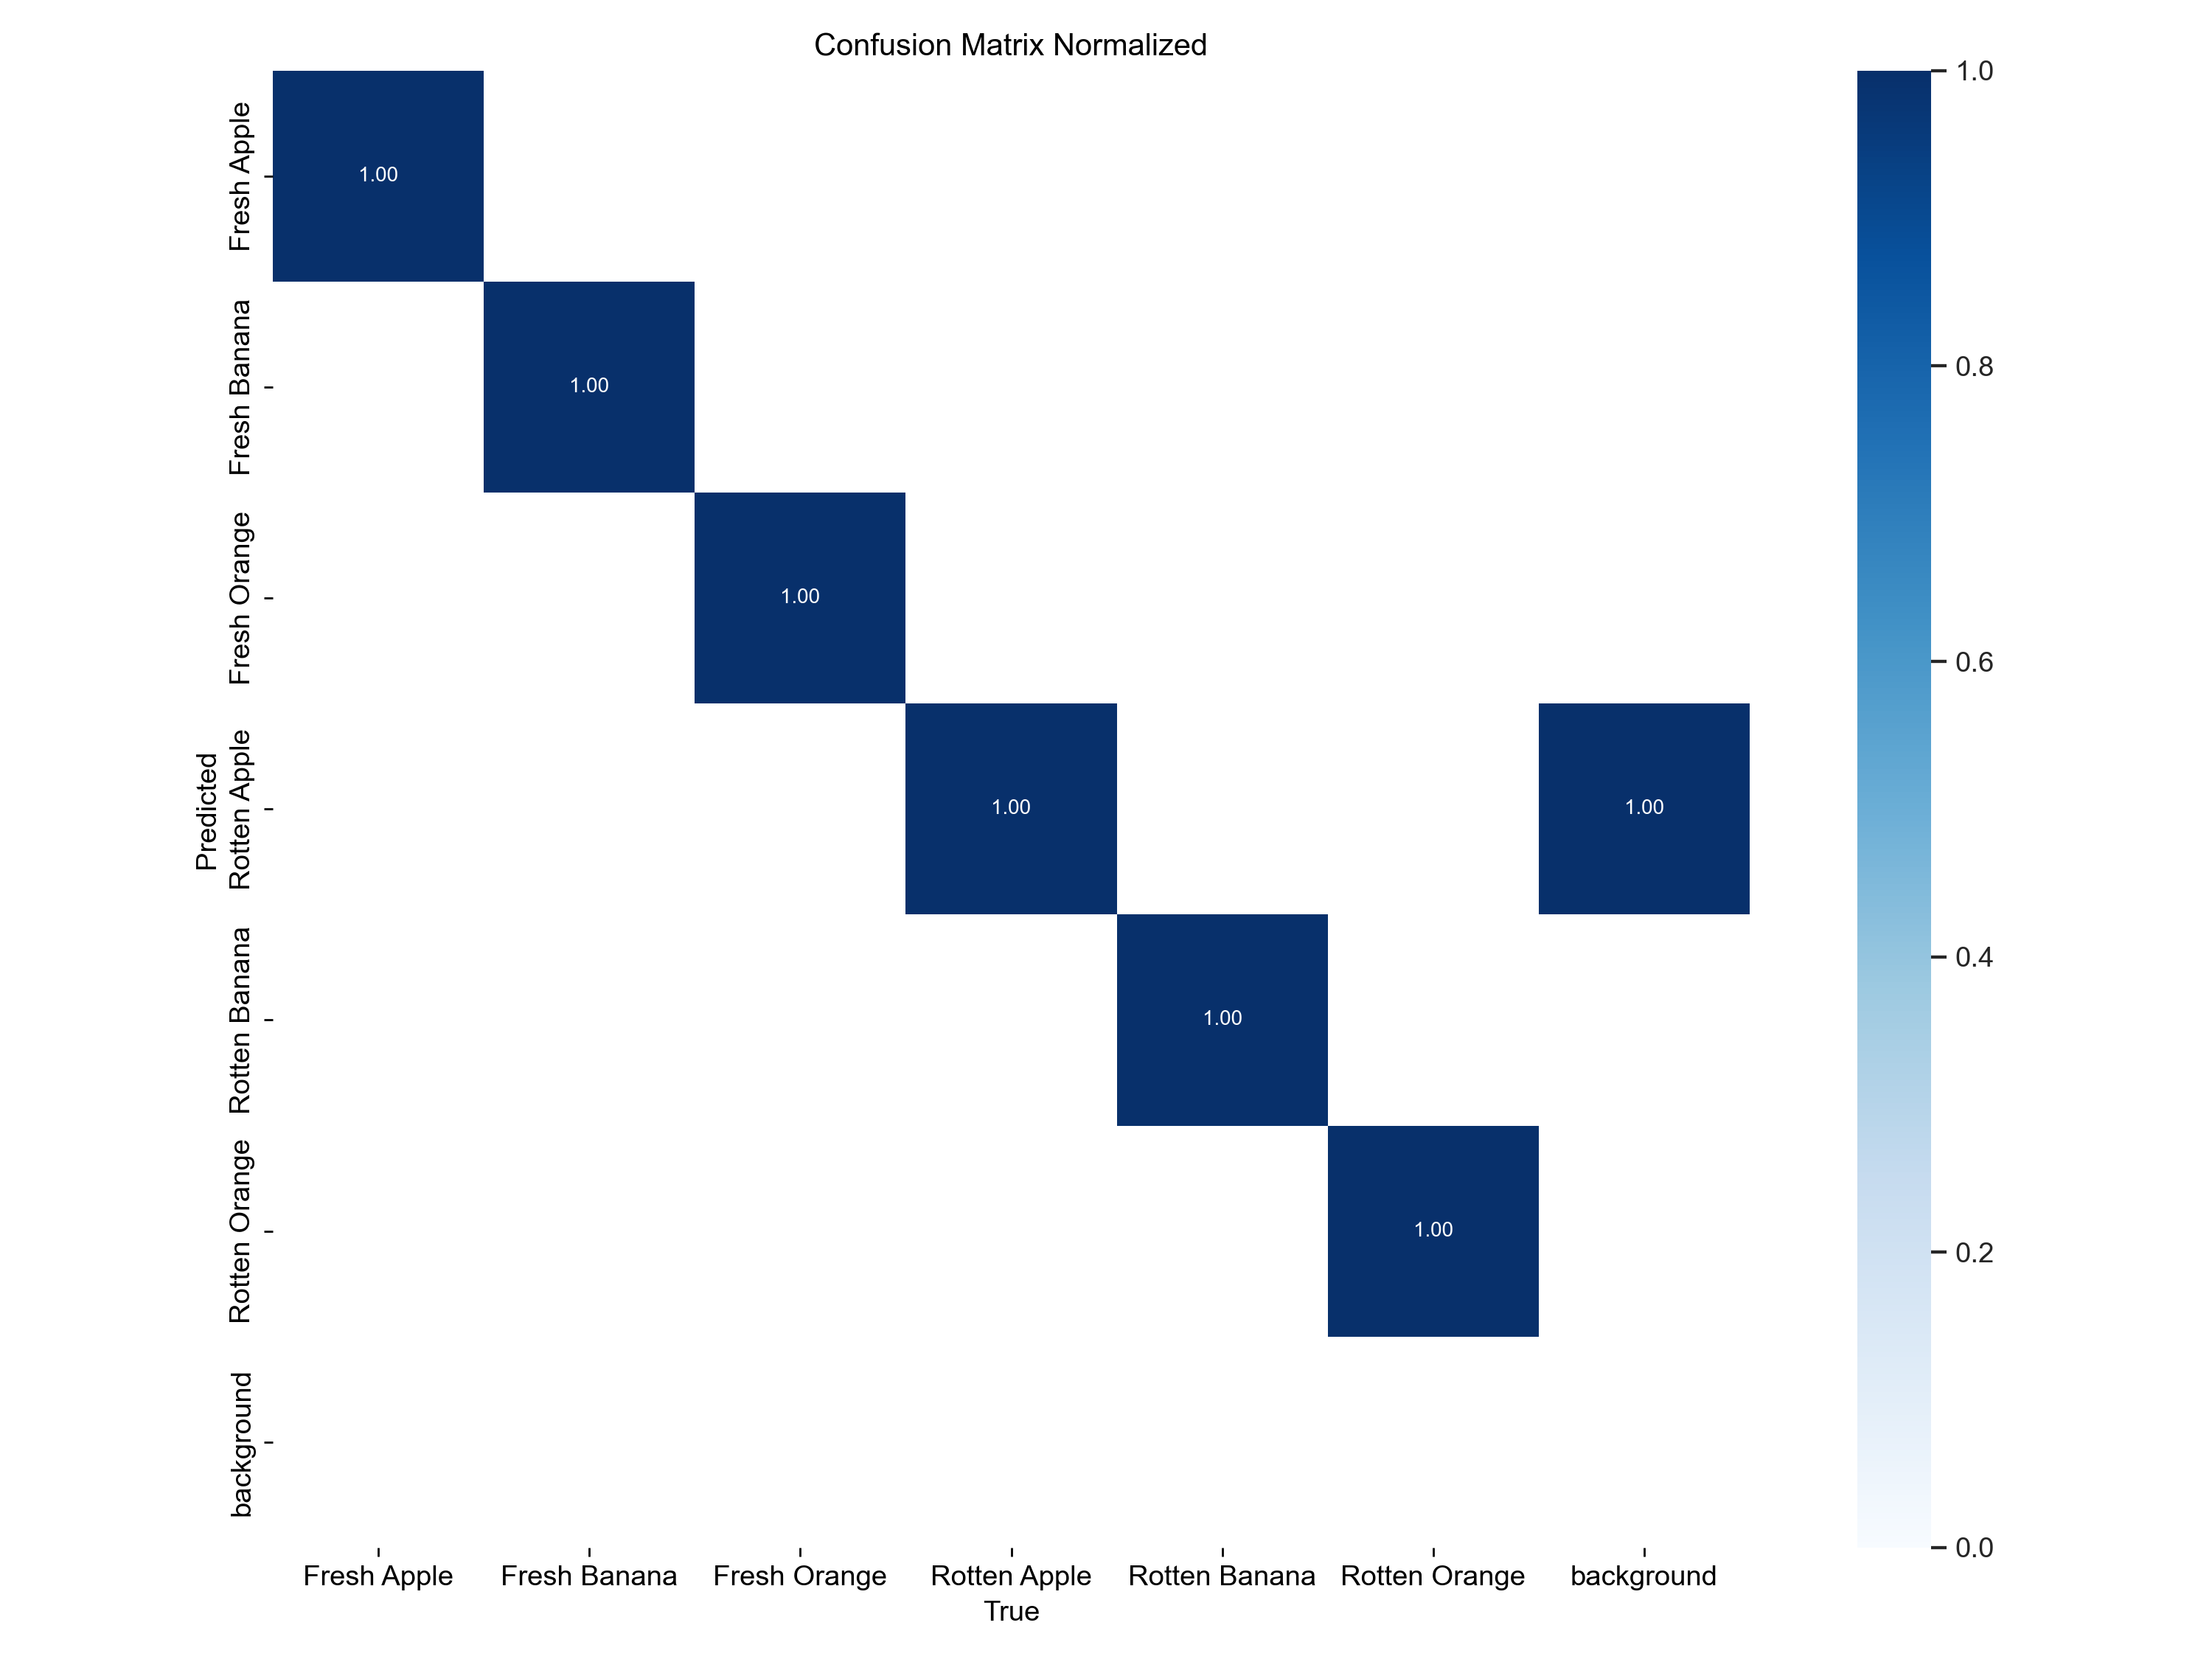
\includegraphics[width=0.95\linewidth]{datas/agriculture/confusion_matrix_normalized.png}
\caption{Confusion Matrix for Fruit Ripeness Classification}
\label{fig:fruit_confusion}
\end{figure}
\begin{multicols}{2}
It's worth noting that despite using the smallest model variant (YOLO v11n), the fruit ripeness detection achieved the highest accuracy, demonstrating that model size is not always the determining factor for performance when the visual features are sufficiently distinctive.

\subsubsection{Cross-Application Performance Comparison}

A comparative analysis of YOLO v11's performance across all three applications reveals substantial performance differences between the medical and agricultural applications, with fruit ripeness detection achieving near-perfect metrics, blood cell detection showing excellent results, and COVID-19 X-ray analysis demonstrating moderate performance.

This pattern suggests that YOLO v11's performance correlates with the visual distinctiveness of the target objects and the complexity of the detection task. Agricultural applications like fruit ripeness detection benefit from clear visual differences between classes, while medical imaging tasks such as COVID-19 detection involve more subtle patterns that are challenging even for human experts.

\subsection{Qualitative Analysis}

Beyond quantitative metrics, we conducted qualitative assessments to understand the models' behavior in different scenarios and identify patterns in successful and failed detections.

\subsubsection{COVID-19 X-ray Detection Analysis}

Visual inspection of the COVID-19 detection results revealed several interesting patterns. The model reliably identified normal X-rays with high confidence. For COVID-19 cases, the model sometimes focused on specific regions like ground-glass opacities but missed more subtle patterns. Confusion between COVID-19 and viral pneumonia typically occurred in cases with extensive bilateral involvement. Edge cases with atypical presentations posed the greatest challenge for the model.

These observations align with the quantitative results and highlight the inherent difficulty of COVID-19 diagnosis from X-rays, which is challenging even for expert radiologists. The model's performance, while not perfect, demonstrates potential as an assistive tool for preliminary screening or workload prioritization in clinical settings.

\subsubsection{Blood Cell Detection Analysis}

Qualitative analysis of blood cell detection results showed excellent performance in most scenarios, with a few notable observations. WBCs were consistently detected with high confidence, likely due to their distinctive size and staining characteristics. RBC detection occasionally struggled in densely packed regions where cells overlap significantly. The model successfully identified platelets despite their smaller size, though with slightly lower confidence than the other cell types. Detection performance remained consistent across different staining intensities and image qualities.

The precision-recall curve (Figure \ref{fig:blood_cell_pr}) shows that the model maintained high precision even at high recall thresholds for all cell types, with WBCs exhibiting the best performance (mAP@50: 0.982) and RBCs showing the most gradual decline in precision as recall increased.
\end{multicols}

\begin{figure}[ht]
\centering
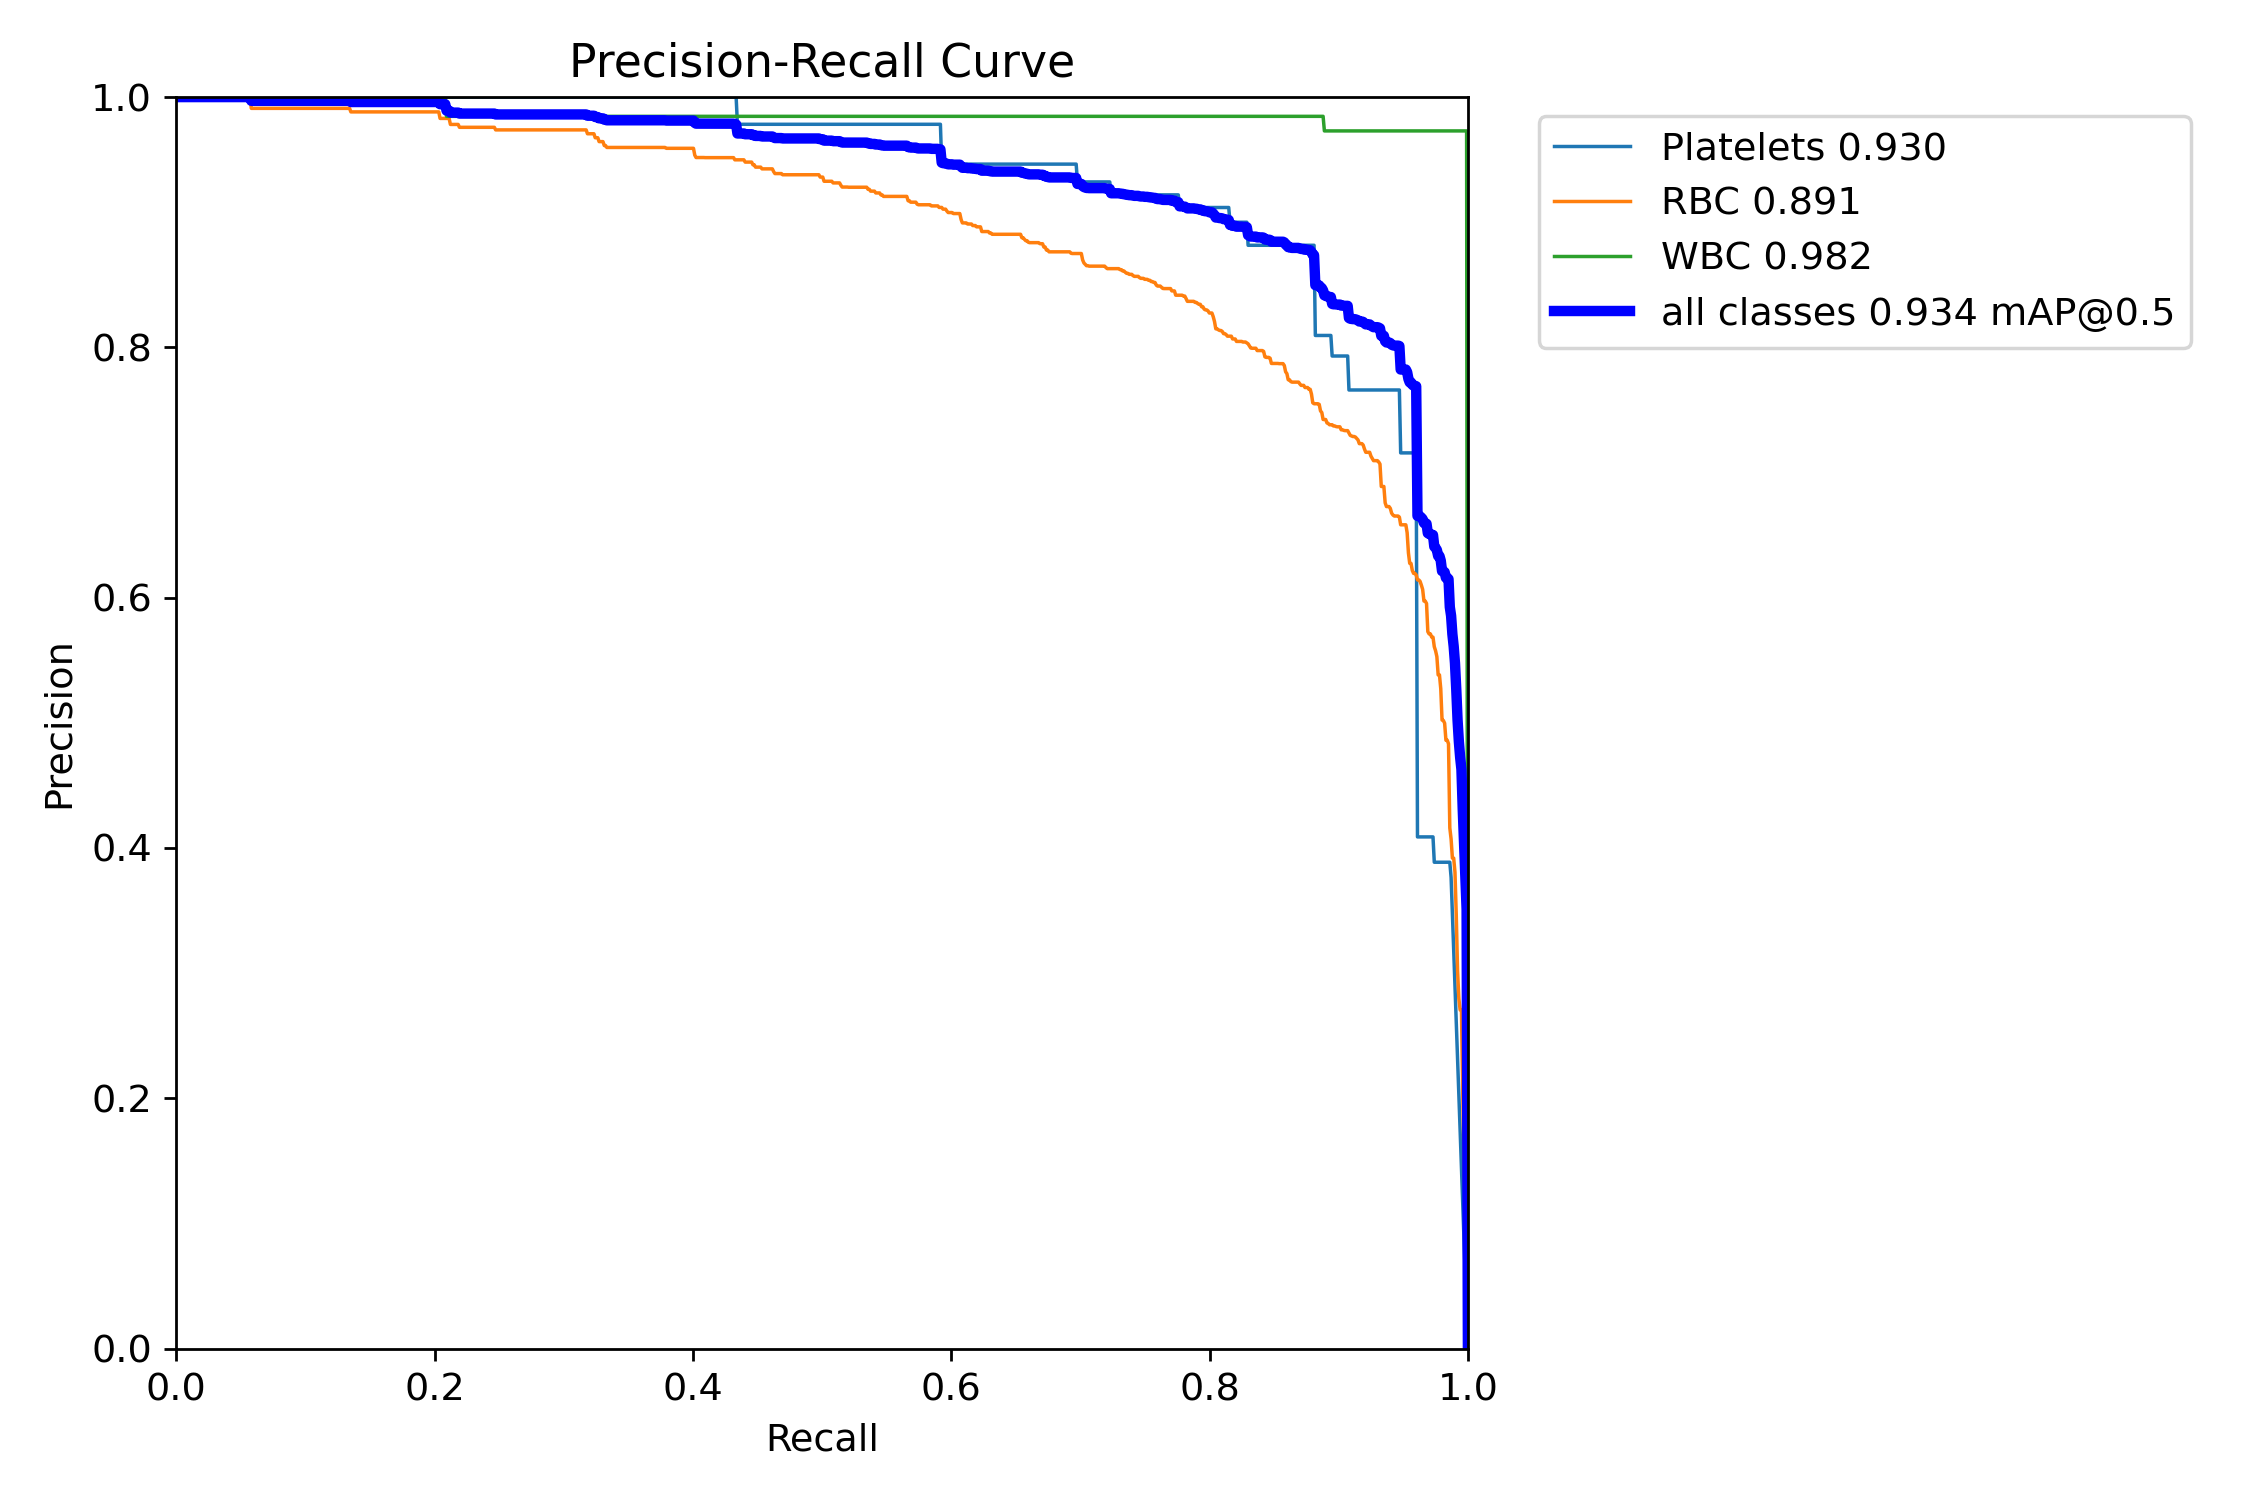
\includegraphics[width=0.8\textwidth]{datas/blood_cell_summary_datas/blood_cells_PR_curve.png}
\caption{Precision-Recall Curve for Blood Cell Detection}
\label{fig:blood_cell_pr}
\end{figure}

\begin{multicols}{2}
\subsubsection{Fruit Ripeness Detection Analysis}

The qualitative analysis of fruit ripeness detection showed exemplary performance across all categories. The model correctly identified all fresh and rotten fruits with high confidence scores (typically > 0.93). Detection remained accurate across various lighting conditions and backgrounds. The R-LBP preprocessing technique effectively highlighted textural changes in rotting fruits, enhancing detection reliability. Even early stages of decay were accurately classified as rotten, demonstrating sensitivity to subtle color and texture changes.

As shown in Figure \ref{fig:fruit_examples}, both fresh and rotten fruits were correctly classified with high confidence scores. The model was particularly effective at detecting the distinctive discoloration and textural changes in rotten fruits, even when these changes were limited to a portion of the fruit.
\end{multicols}

\begin{figure}[ht]
\centering
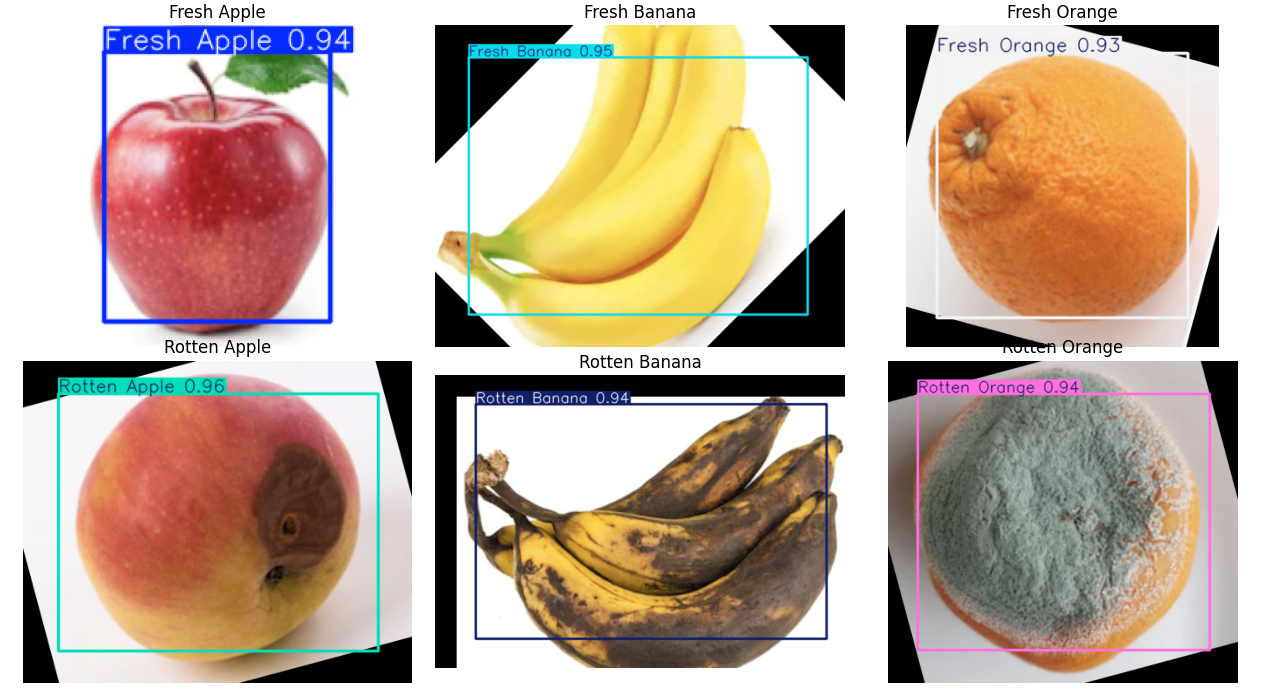
\includegraphics[width=0.8\textwidth]{datas/agriculture/Figure_1.png}
\caption{Example Fruit Ripeness Detection Results}
\label{fig:fruit_examples}
\end{figure}


\begin{figure}[ht]
\centering
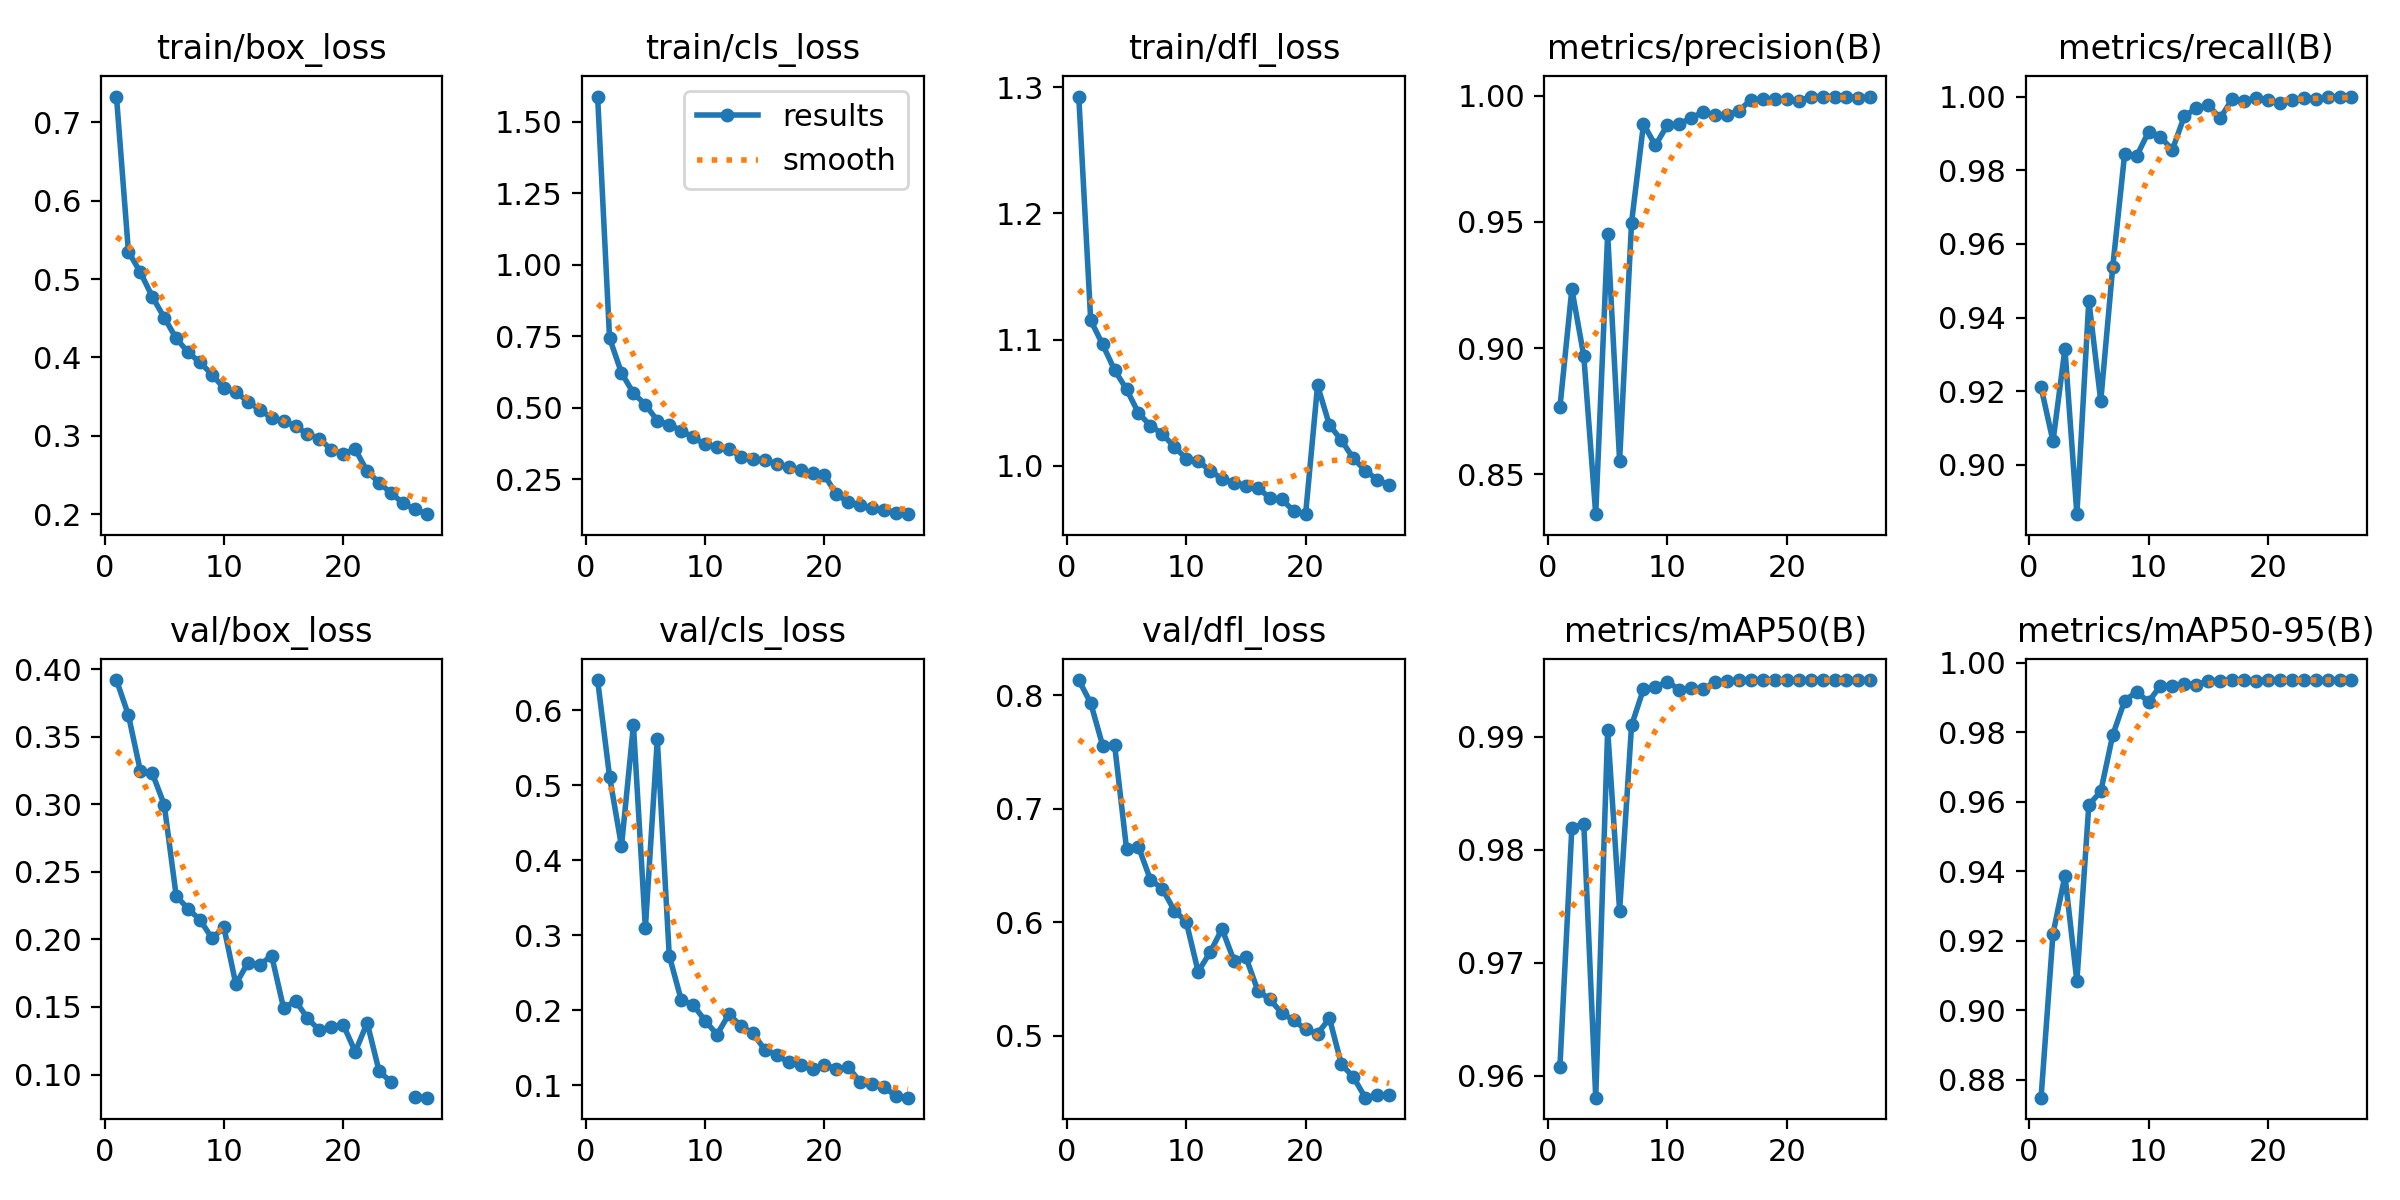
\includegraphics[width=0.82\textwidth]{datas/agriculture/results.png}
\caption{Training Metrics for Fruit Ripeness Detection Model}
\label{fig:fruit_training}
\end{figure}

\begin{multicols}{2}
The mAP@50 and mAP@50-95 metrics showed similar rapid improvement, both exceeding 0.99 by the end of training. This exceptional training efficiency, achieved with the smallest model variant (YOLO v11n), demonstrates the relative simplicity of the fruit ripeness classification task compared to the medical imaging applications.

\subsection{Impact of Model Size and Training Duration}
Our experiments with different YOLO v11 variants (nano, medium, and large) across the three applications provided insights into the relationship between model size, training duration, and performance:

\begin{enumerate}
    \item \textbf{COVID-19 X-ray Detection}: The medium-sized model (YOLO v11m) trained for 20 epochs achieved moderate performance (mAP@50: 0.7263). The limiting factor appeared to be the dataset size and complexity rather than model capacity.
    
    \item \textbf{Blood Cell Detection}: The large model (YOLO v11l) trained for 80 epochs achieved excellent performance (mAP@50: 0.934). The extended training period and larger model capacity were beneficial for this complex task with overlapping objects.
    
    \item \textbf{Fruit Ripeness Detection}: The nano model (YOLO v11n) trained for just 30 epochs achieved near-perfect performance (mAP@50: 0.995). This suggests that for tasks with distinctive visual features, smaller models can be equally effective and more computationally efficient.
\end{enumerate}

These findings indicate that model selection should be guided by the specific characteristics of the detection task rather than simply choosing the largest available model. For deployment in resource-constrained environments, it may be possible to use smaller model variants for certain applications without significant performance degradation.

\subsection{Domain-Specific Challenges and Solutions}

Each application domain presented unique challenges that required specific adaptations and solutions.

\subsubsection{Biomedical Imaging Challenges}

Medical imaging applications like COVID-19 X-ray and blood cell detection faced several domain-specific challenges:

\begin{enumerate}
    \item \textbf{Limited Data Availability}: Medical datasets are often smaller due to privacy concerns and the cost of expert annotation. We addressed this by limiting certain augmentations and carefully monitoring validation performance to prevent overfitting.
    
    \item \textbf{Class Imbalance}: Medical conditions like COVID-19 may be underrepresented in the dataset. We maintained awareness of this limitation in our interpretation of results.
    
    \item \textbf{Subtle Visual Patterns}: Unlike obvious objects in natural images, medical abnormalities often manifest as subtle pattern changes. We found that YOLO v11 could detect some of these patterns but struggled with the most nuanced cases.
    
    \item \textbf{Annotation Consistency}: Medical image annotations require expert knowledge and may have inter-observer variability. We used standardized annotation protocols to minimize inconsistency.
\end{enumerate}

For the blood cell detection task, we analyzed the relationship between cell size and detection accuracy. We found that larger cells (like WBCs) were more accurately detected than smaller cells (like platelets), which informed our data preprocessing and model training strategies.

\subsubsection{Agricultural Imaging Challenges}

The fruit ripeness detection task presented different challenges:

\begin{enumerate}
    \item \textbf{Varying Lighting Conditions}: Agricultural applications often involve images captured under different lighting conditions. The R-LBP preprocessing technique helped normalize these variations.
    
    \item \textbf{Background Complexity}: Fruits may appear against various backgrounds. YOLO v11 proved robust to these variations, consistently detecting and classifying fruits correctly.
    
    \item \textbf{Temporal Progression}: Ripeness exists on a continuum rather than as discrete states. Our model effectively classified these states into binary categories (fresh/rotten) with high confidence.
    
    \item \textbf{Real-time Processing Requirements}: Agricultural applications often require real-time processing for automated sorting systems. The YOLO v11n model achieved impressive processing speeds (5-7ms per image), making it suitable for high-throughput applications.
\end{enumerate}

\subsection{Discussion and Interpretation}

Our comprehensive evaluation across three diverse applications reveals several important insights about YOLO v11's capabilities and limitations.

\subsubsection{Performance Across Domains}

YOLO v11 demonstrated remarkable versatility, achieving strong performance across both biomedical and agricultural domains. However, the performance varied significantly depending on the task characteristics:

\begin{itemize}
    \item \textbf{Best Performance}: Fruit ripeness detection (mAP@50: 0.995, F1: 0.9993)
    \item \textbf{Strong Performance}: Blood cell detection (mAP@50: 0.934, F1: 0.8887)
    \item \textbf{Moderate Performance}: COVID-19 X-ray detection (mAP@50: 0.7263, F1: 0.4349)
\end{itemize}

This performance gradient correlates with task complexity, data availability, and the distinctiveness of visual features. The fruit ripeness task, with its clear visual differences between fresh and rotten fruits, was most amenable to YOLO's detection capabilities. In contrast, the subtle radiological patterns of COVID-19 presented a more challenging scenario, resulting in lower performance despite using a larger model variant.

\subsubsection{Inference Speed and Real-time Capabilities}

All three model configurations achieved inference speeds suitable for real-time or near-real-time applications:

\begin{itemize}
    \item COVID-19 X-ray (YOLO v11m): 33.76 FPS
    \item Blood Cell Detection (YOLO v11l): 38.45 FPS
    \item Fruit Ripeness (YOLO v11n): ~143-200 FPS (5-7ms per image)
\end{itemize}

These speeds make YOLO v11 viable for time-sensitive applications such as automated fruit sorting, intraoperative decision support, or rapid medical screening. Notably, even the largest model variant maintained real-time performance, highlighting YOLO's efficient architecture design.

\subsubsection{Model Size vs. Performance Trade-offs}

Our experiments with different model variants revealed interesting trade-offs between model size and performance:

\begin{itemize}
    \item The nano model (YOLO v11n) achieved the best results on the fruit ripeness task
    \item The medium model (YOLO v11m) showed moderate performance on the COVID-19 task
    \item The large model (YOLO v11l) excelled at the complex blood cell detection task
\end{itemize}

This suggests that model selection should be task-specific rather than defaulting to the largest available variant. For applications with distinctive visual features, smaller models may offer the best balance of performance and computational efficiency.

\subsubsection{Domain-Specific Optimizations}

Each application benefited from domain-specific optimizations:

\begin{itemize}
    \item Medical imaging: Limited rotational augmentation, horizontal flipping only
    \item Blood cell detection: Extended training duration (80 epochs) for fine-grained detection
    \item Fruit ripeness: R-LBP preprocessing for enhanced texture discrimination
\end{itemize}

These optimizations highlight the importance of domain knowledge in achieving optimal performance. The standard YOLO training pipeline can be enhanced significantly through thoughtful adaptation to the specific characteristics of each application domain.

\subsection{Conclusion of Evaluation}

Our comprehensive evaluation demonstrates that YOLO v11 is a versatile object detection framework capable of strong performance across diverse domains, from medical imaging to agricultural applications. The model's performance varies predictably based on task complexity, data availability, and the distinctiveness of visual features:

\begin{enumerate}
    \item \textbf{For agricultural applications} like fruit ripeness detection, YOLO v11 achieves exceptional accuracy with even the smallest model variant, making it an excellent choice for deployment in resource-constrained environments such as embedded systems for automated sorting.
    
    \item \textbf{For blood cell detection}, YOLO v11 provides excellent performance with the large model variant, suggesting its suitability for laboratory automation and computer-aided diagnostics in hematology.
    
    \item \textbf{For COVID-19 X-ray analysis}, YOLO v11 shows promising but moderate performance, indicating potential as an assistive screening tool rather than a standalone diagnostic solution. The model could be valuable for triage and workload prioritization in clinical settings.
\end{enumerate}

These findings advance our understanding of YOLO's capabilities and limitations across different application domains, providing valuable guidance for future implementations in both biomedical and agricultural industries.
\end{multicols}